\documentclass[a4paper,10pt]{article}
\usepackage[cm]{fullpage}
\usepackage{tkz-orm}
\pagestyle{empty}
\usepackage{fancybox}
\begin{document}
\fancypage{\fbox}{}
\sffamily

\def\i#1{\textit{#1}}
\def\b#1{\textbf{#1}}

\tikzset{under/.style={label={[label distance=2mm,font=\itshape,align=center]below:#1}}}

\begin{tikzpicture}[orm]
\matrix[column sep=4mm,label={
  \b{n-ary predicates} are shown as sequence of \i{n} concatenated \b{role}
  boxes. Roles may have \b{role names}.}
]{
  \unary[label=above:died,under=unary]{}; &
  \binary[label=above:wrote,under=binary]{}; &
  \binary[label=above:\ormleft{written by},under={inverse\\reading}]{}; &
  \binary[label=above:owns/owned by,under={both\\readings}]{}; &
  \ternary[label=above:met \ldots at,under=ternary]{}; &
  \node{\i{etc.}}; &
  \entity (p) {Person}; &
  \node[minimum width=10mm]{};
\\ };
\binary[right=of p,label=above:wrote] (w) {};
\plays (p) to (w);
\node[role name,below=of w.one north] {[author]};
\node[fill=white,minimum size=4mm,minimum width=4mm] at (w.east) {};
\end{tikzpicture}

%Each role must be connected to exactely one object type. Only independent
%object types exist without playing any roles.

\begin{tikzpicture}[orm]
\matrix[column sep=0mm,row sep=2.5mm,label={
Each role must be connected to exactely one \b{object type}.
}] {
  & \entity{A}; & \value{A}; & \\
\node[left]{\i{independent}}; &
  \entity{A$^!$}; & \value{A$^!$}; &
  \node[right]{can exist without playing roles}; \\
\node[left]{\i{duplicated}}; & 
  \entity[duplicated]{A}; & \value[duplicated]{A}; & 
  \node[right]{also elsewhere in model}; \\
\node[left]{\i{external}}; & 
  \entity[under=entity]{A$^+$}; & \value[under=value]{A$^+$}; & 
  \node[right]{details excluded from model}; \\
};
\end{tikzpicture}

% TODO: Reference modes

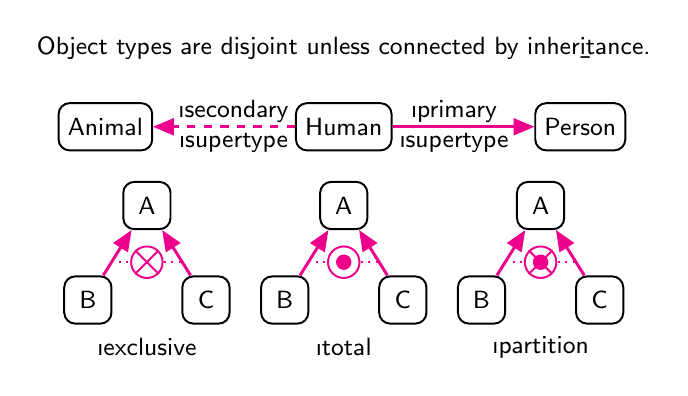
\begin{tikzpicture}[orm,level distance=12mm]
\node at (0,2)
  {Object types are disjoint unless connected by \b{inheritance}.};

\entity (h) at (0,1) {Human};
\entity[right=18mm of h] (p) {Person};
\entity[left=18mm of h] (a) {Animal};
\draw[suptype] (h) to (p);
\draw[supinterface] (h) to (a);
\node[align=left] at (-1.4,1.2) {\i{secondary}};
\node[align=left] at ( 1.4,1.2) {\i{primary}};
\node[align=left] at (-1.4,0.8) {\i{supertype}};
\node[align=left] at ( 1.4,0.8) {\i{supertype}};

\foreach \c/\x in {exclusive/-2.5,total/0,partition/2.5}{
  \entity (A) at (\x,0) {A} [edge from parent/.style=subtype]
    child {node [entity] (B) {B}} child {node [entity] (C) {C}};
  \limits ($(A)!.6!(B)$) to node[constraint=\c] {} ($(A)!.6!(C)$);
  \node at (\x,-1.8) {\i{\c}};
};
\end{tikzpicture}

Not included yet:

\b{uniqueness role constraints} (\i{internal} on one predicate
and \i{external} between different predicates). Further constraints
between roles: \b{exclusion}, \i{exclusive or}, \i{equality},
\i{subset/superset}, \i{equality}, \i{frequency}.
\b{mandatory role constraints}, \b{ring constraints},
\b{value-comparision constraints}, \b{derived fact types},
\b{objectification}, object and role \b{value constraints}.
\b{deontic constraints}, \b{implied model parts}.

\end{document}